\documentclass{article}
\usepackage[left=1cm, right=1cm, top=-0.5cm, bottom=2cm]{geometry}
\usepackage{authblk}
\usepackage{graphicx}

\title{Exploiting LES computations and machine learning to improve wind turbine wake reproduction in URANS}

\author[a]{Andrea Carloni}
\author[a]{Giovanni Delibra}
\author[a]{Valerio Francesco Barnabei}
\author[a]{Alessandro Corsini}
\author[b]{Lorenzo Tieghi}
\author[c]{Filippo De Girolamo}

\affil[a]{Sapienza University of Rome, Rome, Italy}
\affil[b]{Trento University, Trento, Italy}
\affil[c]{KTH Royal Institute of Technology, Stockholm, Sweden}
\date{}

\begin{document}
\maketitle
\begin{abstract}
URANS computations are widely considered unreliable for reproducing wind turbine wake development, limiting their applicability in farm simulations where wake interactions are critical.

This work explores a pipeline combining k-means clustering, to automatically segment the wake into different regions at runtime as in \cite{Carloni2026,Clustering_tieghi}, and neural network regression to derive a machine-learnt correction of eddy viscosity in URANS, based on high-fidelity LES data.

\begin{figure}[h]
    \centering
    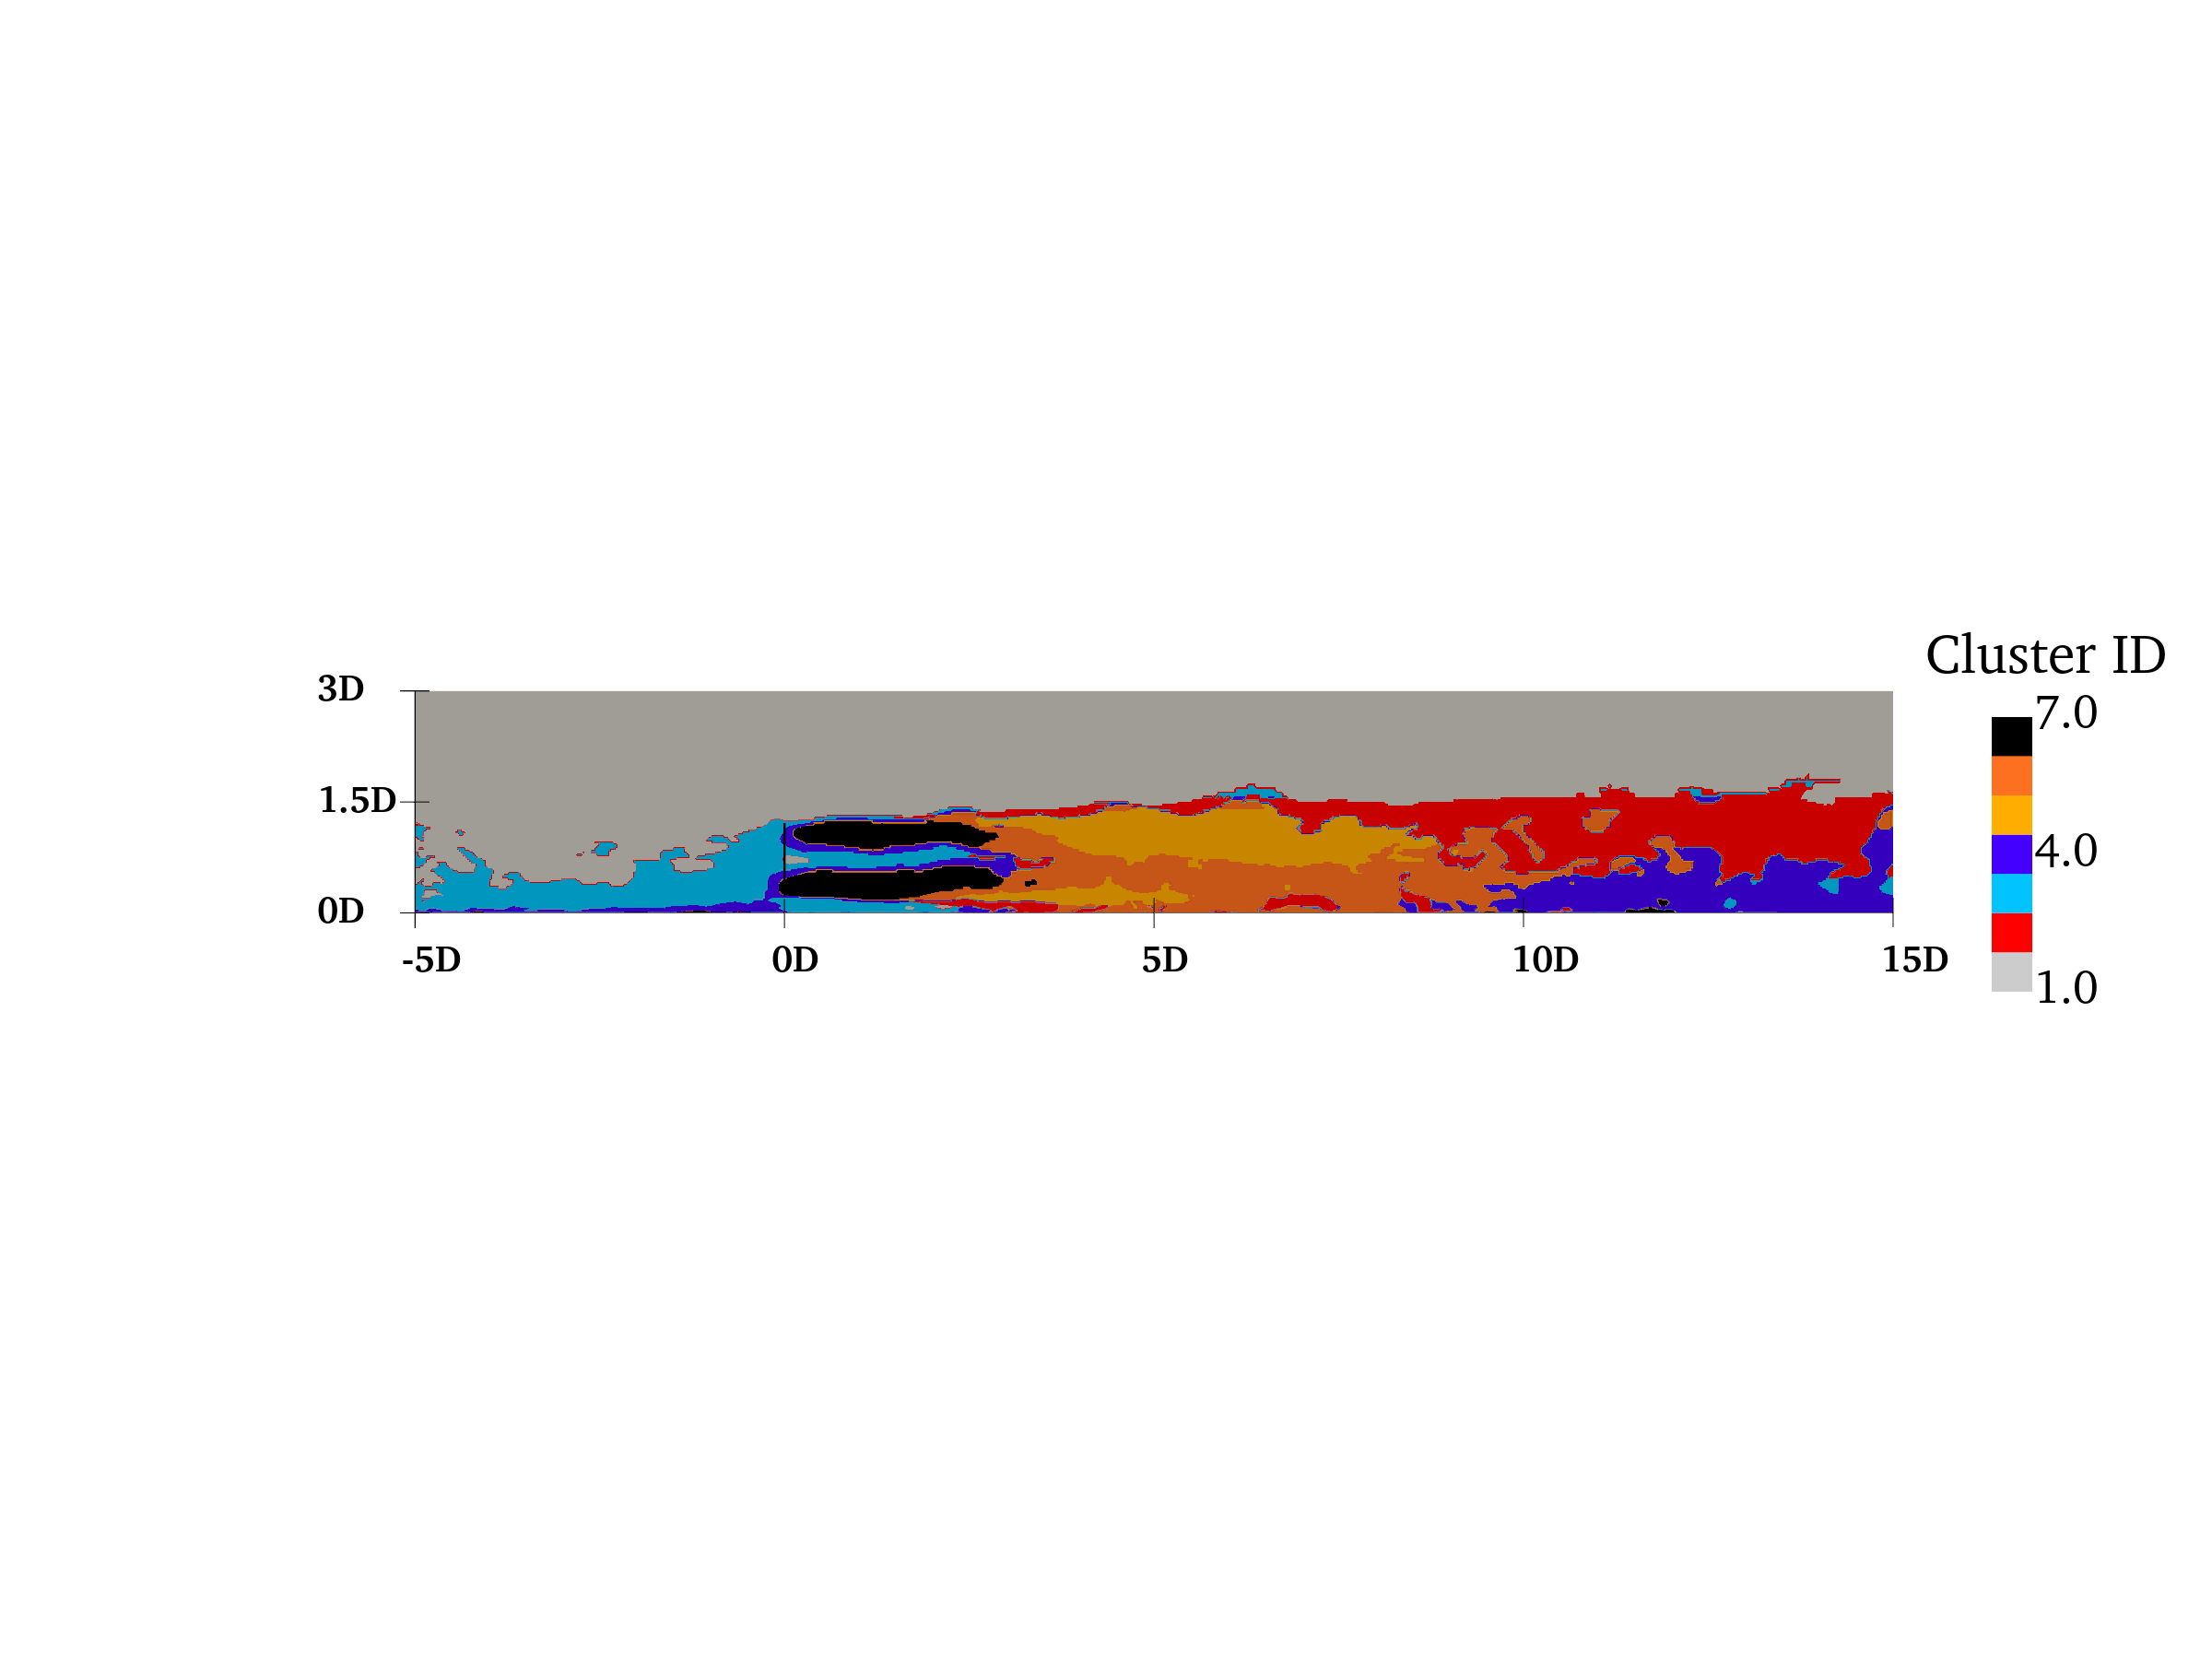
\includegraphics[width=0.8\textwidth, trim = 100 700 0 680, clip]{8ms_0-NC_5final.png}
    \caption{Wake decomposition via clustering \cite{Carloni2026}.}
\end{figure}

LES, RANS, and ML-enhanced RANS simulations are performed in OpenFOAM-v22.12, modelling the NREL 5 MW reference turbine via the Actuator Line Method with a synthetic atmospheric boundary layer at the inflow.

A data-driven correction of RANS eddy viscosity is introduced as an additive term,
\begin{equation}
    \nu_{t,ML}=
    \nu_{t,RANS} +
    \Delta \nu_{t,ML,i},
    \quad i=1,\ldots,N_c ,
\end{equation}
Where $N_c$ is the total number of clusters allowing region-specific eddy-viscosity corrections.
Trained models are embedded in a modified PIMPLE solver, where the eddy viscosity is updated iteratively within the turbulence-correction loop.

\begin{figure}[h]
    \centering
    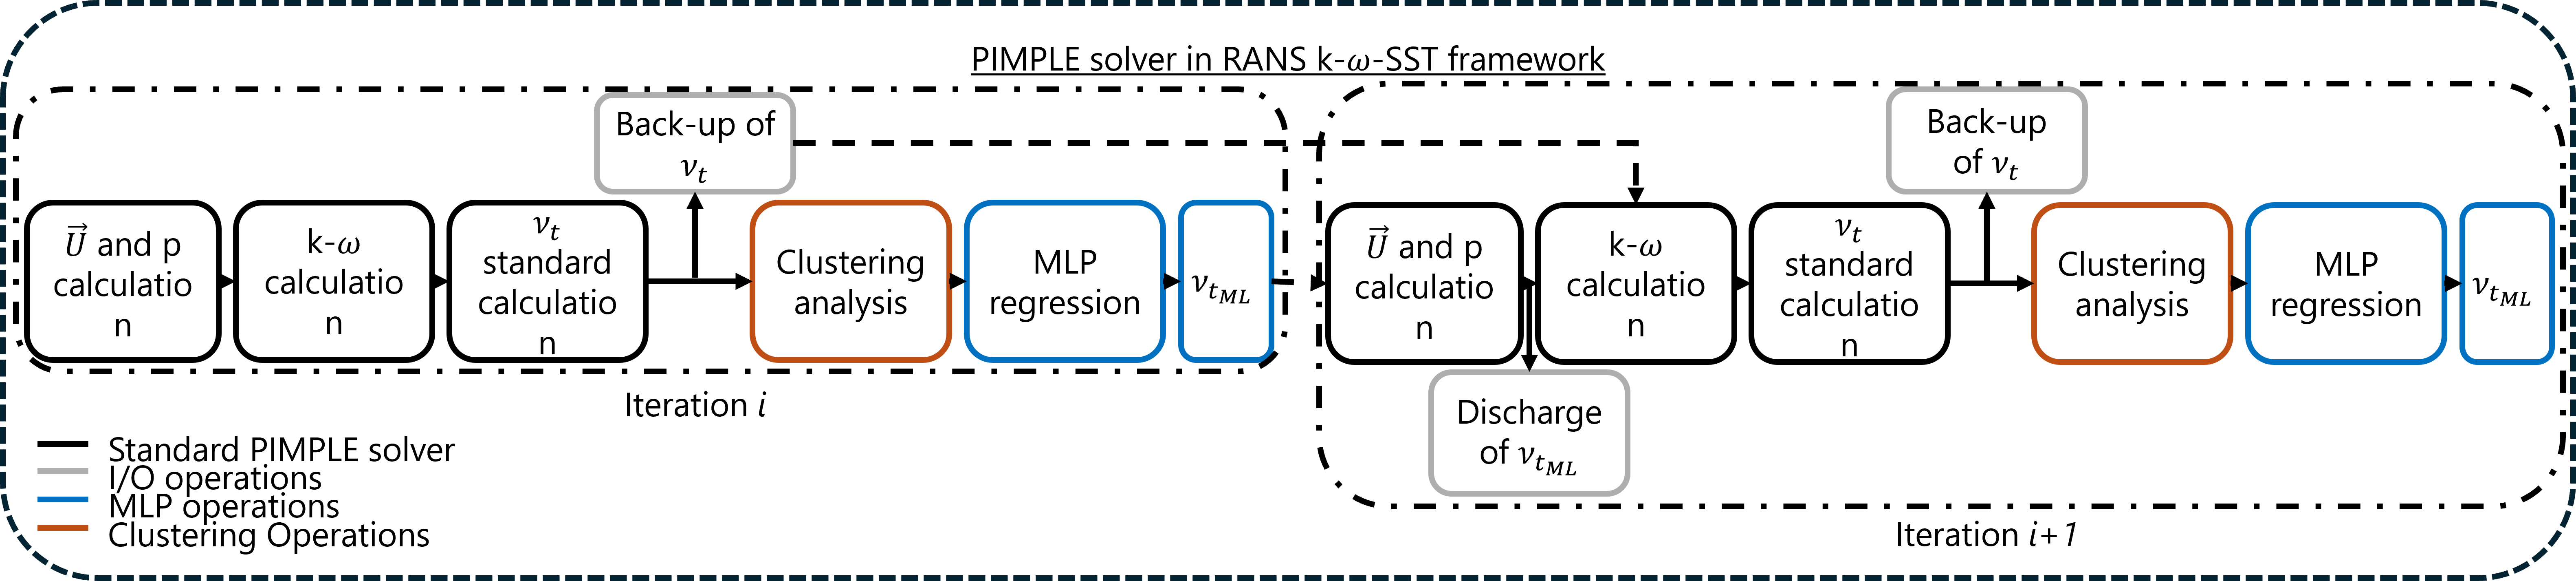
\includegraphics[width=0.8\textwidth]{../methodology/img/solver_pipeline.png}
    \caption{Modified PIMPLE solver pipeline.}
\end{figure}

Results show improved wake-flow prediction over baseline RANS in both near and far wake. The method retains accuracy on grids up to 7$\times$ coarser than LES, yielding substantial computational savings. Non-dimensional topological features support interpretability and generalization to different flow conditions and turbine configurations.

\end{abstract}
\bibliographystyle{unsrt}
\bibliography{ref}
\end{document}
